\documentclass[lettersize,journal]{IEEEtran}
\usepackage{amsmath,amsfonts}
\usepackage{algorithmic}
\usepackage{algorithm}
\usepackage{array}
\usepackage[caption=false,font=normalsize,labelfont=sf,textfont=sf]{subfig}
\usepackage{textcomp}
\usepackage{stfloats}
\usepackage{url}
\usepackage{verbatim}
\usepackage{graphicx}
\usepackage{cite}
\usepackage{booktabs}
\usepackage{multirow}
\usepackage{xcolor}
\usepackage{hyperref}
\usepackage{tikz}
\usetikzlibrary{shapes.geometric, arrows.meta, positioning}
\graphicspath{{figures/}}
\hyphenation{Lang-Graph Lang-Chain Pine-cone}

\begin{document}

\title{Agentic RAG for University Curriculum Navigation: An Empirical Study on Combining Semantic Retrieval with Structured Lookup Tools}

\author{Anh~D.~D.~Hoang, Khang~H.~Tran, ~and~Nam~N.~Trinh
\thanks{The authors are with Information Technology Specialization, FPT University, Hanoi, Vietnam.}
\thanks{Manuscript prepared March 2026.}}

\markboth{DAP391m}%
{Hoang: Agentic RAG for University Curriculum Navigation}

\maketitle

\begin{abstract}
This paper presents the design, implementation, and evaluation of a Retrieval-Augmented Generation (RAG) chatbot that serves as an academic advisor for FPT University's Bachelor of IT in Artificial Intelligence (BIT\_AI) program. The system combines semantic vector search over course syllabi with deterministic structured lookup tools for prerequisite chains, specialization pathways, and semester-level curriculum data. An agentic loop built on LangGraph enables the model to call multiple tools iteratively before synthesizing an answer. We evaluate the system on a 48-question golden test set across five categories using LLM-as-judge metrics. The RAG system achieves a correctness score of 0.625 compared to 0.240 for a baseline LLM-only system (160.4\% relative improvement) and a faithfulness score of 0.865 versus 0.000 for the baseline. Per-category analysis shows the largest correctness gains in factual lookup (+0.550) and combo pathway navigation (+0.500) tasks.
\end{abstract}

\begin{IEEEkeywords}
Retrieval-Augmented Generation, LangGraph, curriculum advising, agentic AI, LLM evaluation.
\end{IEEEkeywords}

% ======================================================================
\section{Introduction}
\IEEEPARstart{U}{niversity} students frequently need guidance navigating complex curricula --- understanding prerequisite chains, choosing specialization pathways, planning course loads, and determining which courses to retake. Traditional advising relies on human counselors who may be unavailable or unfamiliar with the latest curriculum changes. Large Language Models (LLMs) can provide conversational interfaces but hallucinate factual details such as credit counts, semester placements, and prerequisite relationships when operating without access to ground-truth data~\cite{ref_rag_survey}.

Retrieval-Augmented Generation (RAG) addresses this by grounding LLM responses in retrieved documents~\cite{ref_lewis_rag}. However, a standard RAG pipeline with a single vector search step has limitations for structured academic data: prerequisite chains require recursive resolution, semester-course mappings are tabular, and specialization pathways follow a fixed schema. These queries are better served by deterministic lookups than by semantic similarity.

This work presents an \textbf{Agentic RAG} system that combines semantic vector search with structured JSON lookup tools, orchestrated by a LangGraph~\cite{ref_langgraph} state machine. The agent decides which tools to invoke, can call multiple tools in sequence, and includes a document relevance grading step with query rewriting. We evaluate the system against a no-retrieval baseline on a curated 48-question test set covering the BIT\_AI K20-K21 curriculum at FPT University.

The contributions of this paper are:
\begin{enumerate}
    \item A hybrid retrieval architecture combining vector search with four structured lookup tools for academic curriculum data.
    \item A LangGraph-based agentic loop with document grading and multi-tool iteration.
    \item An empirical evaluation comparing RAG versus LLM-only on faithfulness, relevancy, and correctness across five question categories.
\end{enumerate}

% ======================================================================
\section{Related Work}

RAG was introduced by Lewis et al.~\cite{ref_lewis_rag} to mitigate LLM hallucination by conditioning generation on retrieved passages. Subsequent work explored advanced retrieval strategies including re-ranking~\cite{ref_reranking}, query decomposition, and hybrid search. Gao et al.~\cite{ref_rag_survey} provide a comprehensive survey of RAG techniques and their applications.

\textbf{Agentic RAG.} ReAct~\cite{ref_react} introduced the paradigm of interleaving reasoning and tool use in LLMs. LangGraph~\cite{ref_langgraph} operationalizes this pattern with a state machine abstraction, enabling conditional routing, tool invocation, and iterative refinement loops. Our work adopts this architecture for multi-tool academic advising.

\textbf{LLM-as-Judge Evaluation.} Zheng et al.~\cite{ref_llm_judge} demonstrated that LLMs can serve as reliable evaluators of open-ended generation quality, correlating well with human judgments. We use GPT-4o-mini as a judge to score answer relevancy, faithfulness, and correctness.

\textbf{Educational AI.} Prior work on AI tutoring systems~\cite{ref_edu_ai} has focused on content delivery and assessment. Our system targets curriculum navigation specifically --- a planning-oriented task that requires combining information across multiple structured data sources.

% ======================================================================
\section{System Architecture}

\subsection{Data Corpus}

The raw corpus consists of 9 markdown files covering the BIT\_AI K20-K21 curriculum:
\begin{itemize}
    \item \textbf{Syllabi}: Individual course files containing descriptions, learning outcomes, session schedules, assessment structures, and materials.
    \item \textbf{Curriculum}: A master document listing all 47 courses across 10 semesters (semesters 0--9) with credit counts and prerequisites.
    \item \textbf{Pathways}: Specialization combo definitions with elective course groupings organized by topic.
\end{itemize}

Each file is classified by regex matching on its H1 header into one of three entity types: \texttt{syllabus}, \texttt{curriculum}, or \texttt{pathway}.

\subsection{Ingestion Pipeline}

The ingestion pipeline transforms raw markdown into two parallel representations:

\textbf{Vector index.} Documents are split using a \texttt{MarkdownHeaderTextSplitter} at H2 section boundaries, then oversized chunks are sub-split with a \texttt{RecursiveCharacterTextSplitter} (chunk size 500 characters, overlap 50). A minimum chunk length filter of 50 characters removes fragments from table-row splits, reducing the total from 8{,}446 to 6{,}256 chunks. Chunks are embedded with OpenAI \texttt{text-embedding-3-small} (1{,}536 dimensions) and indexed in Pinecone Serverless (cosine similarity).

\textbf{Structured tables.} Six JSON lookup tables are extracted deterministically from the parsed documents:
\begin{enumerate}
    \item \texttt{course\_index}: 47 entries mapping course codes to name, credits, semester, prerequisite, and description.
    \item \texttt{prerequisites}: 23 entries mapping course codes to their prerequisite strings.
    \item \texttt{curriculum\_map}: 10 semesters, each with a list of courses.
    \item \texttt{combo\_map}: 5 specialization pathways with course groupings.
    \item \texttt{programme\_outcomes}: 5 program-level outcomes.
    \item \texttt{program\_learning\_outcomes}: 13 PLOs.
\end{enumerate}

\subsection{Tool Definitions}

Four LangChain tools are defined, each backed by either the vector index or the JSON tables:

\begin{enumerate}
    \item \textbf{vector\_search}$(q, c, t)$: Semantic search over Pinecone. Accepts optional \texttt{course\_code} $c$ for metadata filtering and \texttt{entity\_type} $t \in \{\text{syllabus}, \text{curriculum}, \text{pathway}\}$. Returns top-$k$ ($k{=}5$) chunks with source metadata.
    \item \textbf{prerequisite\_lookup}$(c, d)$: Deterministic prerequisite resolver. Direction $d{=}\text{forward}$ returns the full recursive prerequisite chain; $d{=}\text{reverse}$ finds courses that list $c$ as a prerequisite.
    \item \textbf{combo\_navigator}$(id, t)$: Browse specialization pathways by ID or topic name search. Returns course listings with active/inactive status.
    \item \textbf{curriculum\_browser}$(s, c)$: Browse the study plan by semester $s$ or look up a specific course $c$. Returns course names, credits, and prerequisites.
\end{enumerate}

All tools include a fuzzy course code resolver that handles partial input (e.g., ``AIL'' $\rightarrow$ ``AIL303m'') via prefix matching against the course index.

\subsection{LangGraph Agent}

The agent is implemented as a LangGraph \texttt{StateGraph} with four nodes and conditional routing:

\begin{algorithm}[H]
\caption{Agent graph execution.}\label{alg:agent}
\begin{algorithmic}
\STATE $s \gets$ \textsc{InitState}(question, history, profile)
\REPEAT
    \STATE $response \gets$ \textsc{AgentNode}($s$) \hfill \textit{// LLM with tools}
    \IF{$response$ has tool calls}
        \STATE $results \gets$ \textsc{ToolNode}($response$.tool\_calls)
        \STATE $grade \gets$ \textsc{GradeDocuments}($results$)
        \IF{$grade = $ not\_relevant \AND retries $< 1$}
            \STATE Rewrite query, increment retry
        \ENDIF
        \STATE Increment tool\_call\_count
    \ENDIF
\UNTIL{no tool calls \OR tool\_call\_count $\geq 6$}
\STATE $answer \gets$ \textsc{GenerateNode}(current\_turn\_messages)
\RETURN $answer$
\end{algorithmic}
\end{algorithm}

Fig.~\ref{fig:agent_graph} illustrates the graph structure visually.

\begin{figure}[!t]
\centering
\resizebox{\columnwidth}{!}{%
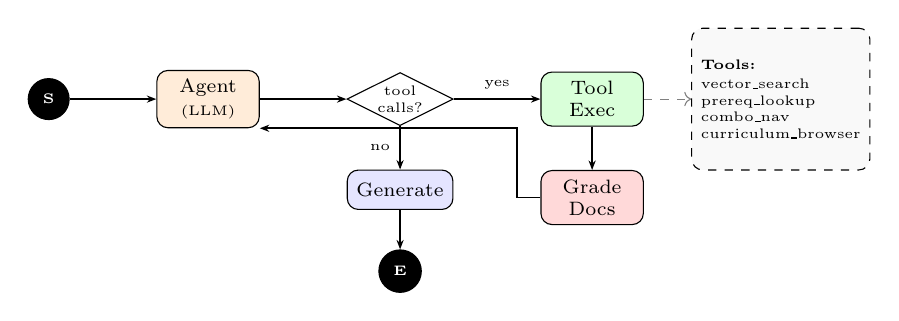
\begin{tikzpicture}[
    node distance=0.65cm and 1.1cm,
    every node/.style={font=\scriptsize},
    process/.style={rectangle, rounded corners, draw, minimum width=1.3cm, minimum height=0.5cm, align=center},
    decision/.style={diamond, draw, aspect=2, inner sep=0.5pt, align=center, font=\tiny},
    startstop/.style={circle, draw, fill=black, text=white, minimum size=0.4cm, font=\tiny\bfseries},
    arrow/.style={-{Stealth[length=1.2mm]}, semithick},
]

\node[startstop] (start) {S};
\node[process, fill=orange!15, right=of start] (agent) {Agent\\{\tiny(LLM)}};
\node[decision, right=of agent] (hastools) {tool\\calls?};
\node[process, fill=green!15, right=of hastools] (tools) {Tool\\Exec};
\node[process, fill=red!15, below=0.55cm of tools] (grade) {Grade\\Docs};
\node[process, fill=blue!10, below=0.55cm of hastools] (generate) {Generate};
\node[startstop, below=0.5cm of generate] (end) {E};

\draw[arrow] (start) -- (agent);
\draw[arrow] (agent) -- (hastools);
\draw[arrow] (hastools) -- node[above, font=\tiny] {yes} (tools);
\draw[arrow] (hastools) -- node[left, font=\tiny] {no} (generate);
\draw[arrow] (tools) -- (grade);
\draw[arrow] (grade.west) -- +(-0.3,0) |- (agent.south east);
\draw[arrow] (generate) -- (end);

\node[draw, dashed, rounded corners, fill=gray!5,
      right=0.6cm of tools, minimum width=1.8cm, minimum height=1.8cm, align=left, font=\tiny] (toolbox) {
    \textbf{Tools:}\\[0.15em]
    vector\_search\\
    prereq\_lookup\\
    combo\_nav\\
    curriculum\_browser
};

\draw[dashed, ->, gray] (tools.east) -- (toolbox.west);

\end{tikzpicture}%
}
\caption{LangGraph agent state machine. The agent--tools--grade loop repeats up to 6 iterations. Structured tools bypass grading; only \texttt{vector\_search} results are graded for relevance.}
\label{fig:agent_graph}
\end{figure}

Structured tools (prerequisite\_lookup, combo\_navigator, curriculum\_browser) skip the grading step since they return deterministic data. Only \texttt{vector\_search} results are graded for relevance by an LLM judge, with one query rewrite attempt if irrelevant.

The \textsc{GenerateNode} receives only the current turn's messages (extracted by walking backward to the last \texttt{HumanMessage}) to prevent prior conversation turns from bleeding into the response.

\subsection{Student Personalization}

The system supports student profiles containing passed courses with grades, failed courses, and current semester. Profile data is injected into the system prompt as structured context. The agent cross-references this with tool results to provide personalized advice: flagging blocked courses due to failed prerequisites, suggesting retake candidates, and building acceleration plans respecting FPT's rule of at most 2 extra courses per semester from the next semester.

% ======================================================================
\section{Experimental Setup}

\subsection{Test Set}

We curated a golden test set of 48 question--answer pairs across five categories:

\begin{table}[!t]
\caption{Golden Test Set Composition\label{tab:testset}}
\centering
\begin{tabular}{lrl}
\toprule
\textbf{Category} & \textbf{Count} & \textbf{Example Question Type} \\
\midrule
Factual Lookup & 10 & Course credits, semester placement \\
Prerequisite Reasoning & 10 & Dependency chains, reverse lookup \\
Combo Pathway & 8 & Specialization courses, electives \\
Cross Document & 10 & Multi-source synthesis \\
Curriculum Planning & 10 & Acceleration, semester planning \\
\midrule
\textbf{Total} & \textbf{48} & \\
\bottomrule
\end{tabular}
\end{table}

Each entry includes a reference answer, expected tool, and expected sources for evaluation grounding.

\subsection{Metrics}

We use LLM-as-judge evaluation~\cite{ref_llm_judge} with GPT-4o-mini scoring three metrics on a $[0, 1]$ scale:
\begin{itemize}
    \item \textbf{Answer Relevancy}: Does the answer address the question asked?
    \item \textbf{Faithfulness}: Is the answer grounded in the retrieved context (not hallucinated)?
    \item \textbf{Correctness}: Does the answer match the reference answer?
\end{itemize}

\subsection{Systems Under Evaluation}

\textbf{RAG system}: The full agentic pipeline with all four tools, document grading, and query rewriting. Uses GPT-4o-mini (\texttt{temperature=0}) for both agent reasoning and final generation.

\textbf{Baseline}: GPT-4o-mini with a minimal system prompt (``You are an academic advisor for FPT University's BIT\_AI program'') and no access to tools or retrieval. This isolates the improvement attributable to RAG.

Both systems were evaluated on all 48 questions. Tool calls, generated answers, and judge scores with reasoning were recorded for each question.

% ======================================================================
\section{Results}

\subsection{Overall Performance}

Table~\ref{tab:overall} summarizes the aggregate metrics across all 48 questions.

\begin{table}[!t]
\caption{Overall Evaluation Metrics\label{tab:overall}}
\centering
\begin{tabular}{lccc}
\toprule
\textbf{Metric} & \textbf{RAG} & \textbf{Baseline} & \textbf{$\Delta$} \\
\midrule
Relevancy & 0.958 & 0.948 & +0.010 \\
Faithfulness & 0.865 & 0.000 & +0.865 \\
Correctness & 0.625 & 0.240 & +0.385 \\
\bottomrule
\end{tabular}
\end{table}

The RAG system achieves a correctness score 160.4\% higher than the baseline in relative terms (+0.385 absolute). Faithfulness improves from 0.000 to 0.865 --- the baseline receives a score of zero because it has no context to be faithful to, while the RAG system grounds its answers in tool results. Relevancy is comparable between the two systems (0.958 vs.\ 0.948), indicating that both understand the questions well; the difference lies in answer accuracy.

Fig.~\ref{fig:overall} visualizes this comparison.

\begin{figure}[!t]
\centering
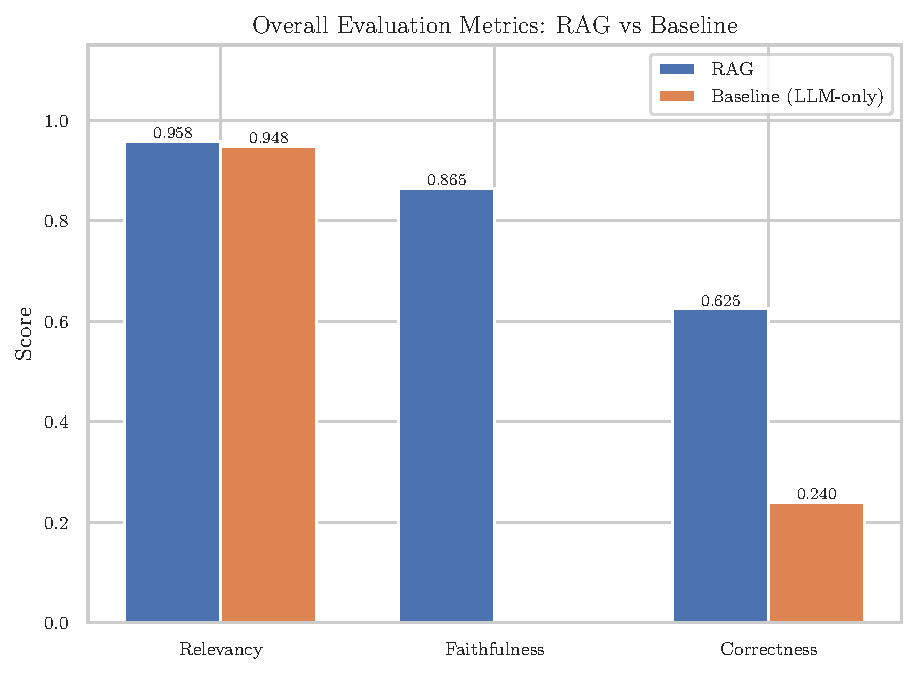
\includegraphics[width=\columnwidth]{overall_comparison.pdf}
\caption{Overall evaluation metrics comparing the RAG system with the LLM-only baseline across all 48 test questions.}
\label{fig:overall}
\end{figure}

\subsection{Per-Category Analysis}

Table~\ref{tab:category} breaks down correctness scores by question category.

\begin{table}[!t]
\caption{Correctness by Question Category\label{tab:category}}
\centering
\begin{tabular}{lccc}
\toprule
\textbf{Category} & \textbf{RAG} & \textbf{Baseline} & \textbf{$\Delta$} \\
\midrule
Factual Lookup & 0.700 & 0.150 & +0.550 \\
Combo Pathway & 0.688 & 0.188 & +0.500 \\
Prerequisite Reasoning & 0.600 & 0.150 & +0.450 \\
Curriculum Planning & 0.600 & 0.250 & +0.350 \\
Cross Document & 0.550 & 0.450 & +0.100 \\
\bottomrule
\end{tabular}
\end{table}

\begin{figure}[!t]
\centering
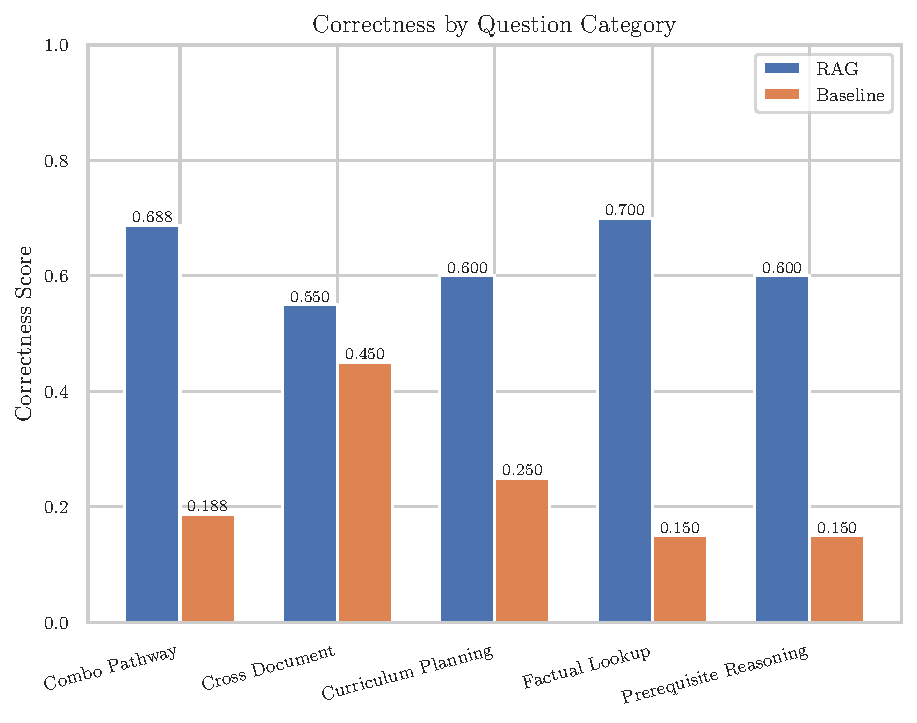
\includegraphics[width=\columnwidth]{category_correctness.pdf}
\caption{Per-category correctness scores. The RAG system shows the largest improvements in Factual Lookup and Combo Pathway categories.}
\label{fig:category}
\end{figure}

The largest improvements appear in \textbf{Factual Lookup} (+0.550) and \textbf{Combo Pathway} (+0.500), where the baseline frequently hallucinates incorrect credit counts, semester placements, and course codes. The smallest improvement is in \textbf{Cross Document} (+0.100), where both systems achieve moderate scores. This category requires synthesizing information across multiple documents, a task where vector search retrieval is less precise because the query must match content scattered across different files.

\subsection{Faithfulness and Correctness Impact}

Fig.~\ref{fig:faithfulness} isolates the impact of retrieval on faithfulness and correctness.

\begin{figure}[!t]
\centering
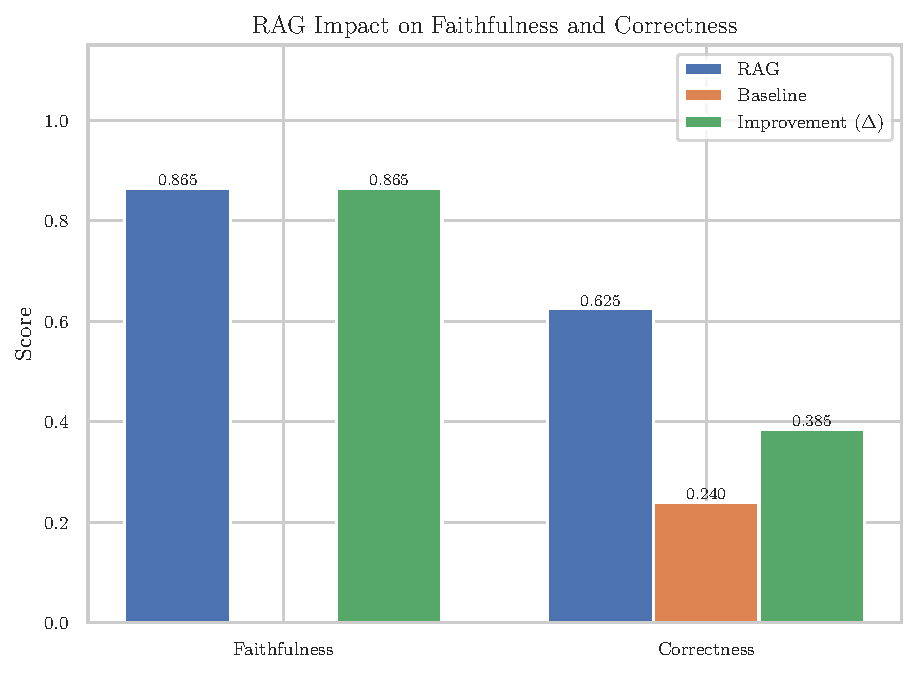
\includegraphics[width=\columnwidth]{faithfulness_impact.pdf}
\caption{RAG impact on faithfulness and correctness. The baseline achieves zero faithfulness because it has no retrieved context to be faithful to.}
\label{fig:faithfulness}
\end{figure}

The faithfulness gap (0.865 vs.\ 0.000) demonstrates that tool access is necessary for grounded answers. The baseline LLM generates plausible-sounding but unsupported claims --- for example, stating that a course has 3 credits when it actually has 6, or placing a course in semester 6 when it belongs to semester 4.

\subsection{Score Distribution}

Fig.~\ref{fig:distribution} shows the distribution of per-question correctness scores for both systems.

\begin{figure*}[!t]
\centering
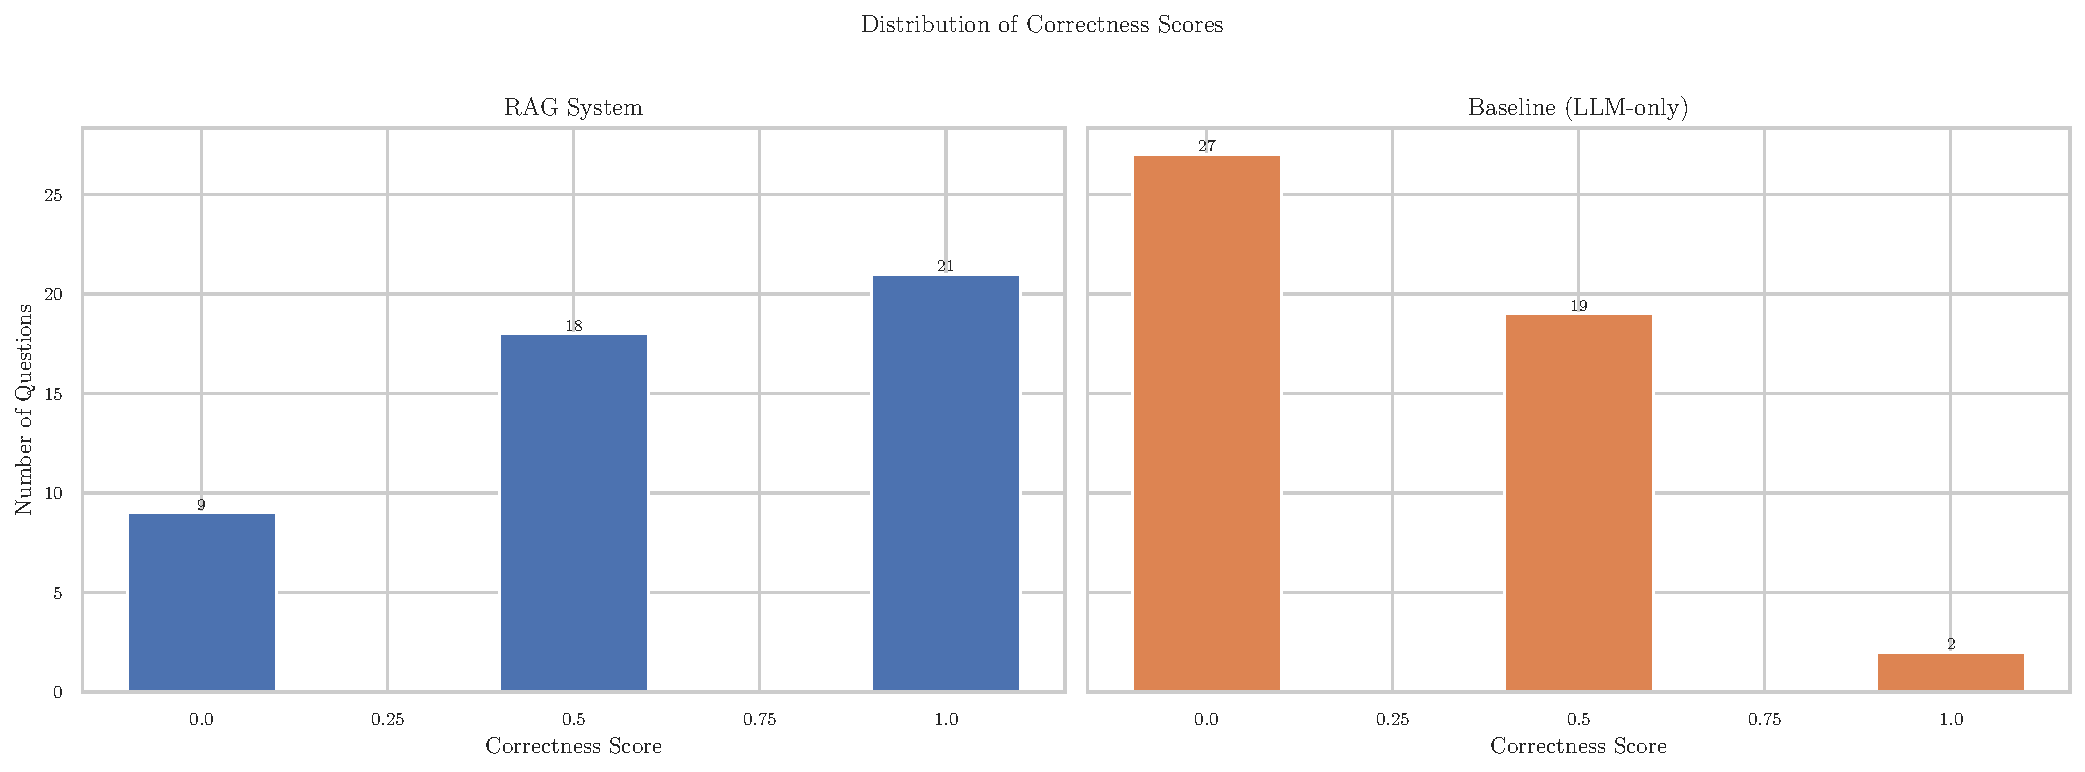
\includegraphics[width=\textwidth]{score_distribution.pdf}
\caption{Distribution of correctness scores across all 48 questions. The RAG system produces more fully correct (1.0) answers and fewer failures (0.0) than the baseline.}
\label{fig:distribution}
\end{figure*}

The RAG system produces 19 fully correct answers (score = 1.0) compared to 5 for the baseline. Conversely, the RAG system has 9 failures (score = 0.0) versus 27 for the baseline. The baseline is concentrated at 0.0 and 0.5, while the RAG system shifts the distribution rightward toward higher correctness.

\subsection{Tool Usage Patterns}

Fig.~\ref{fig:tools} shows the frequency of each tool's invocation across the 48 evaluation questions.

\begin{figure}[!t]
\centering
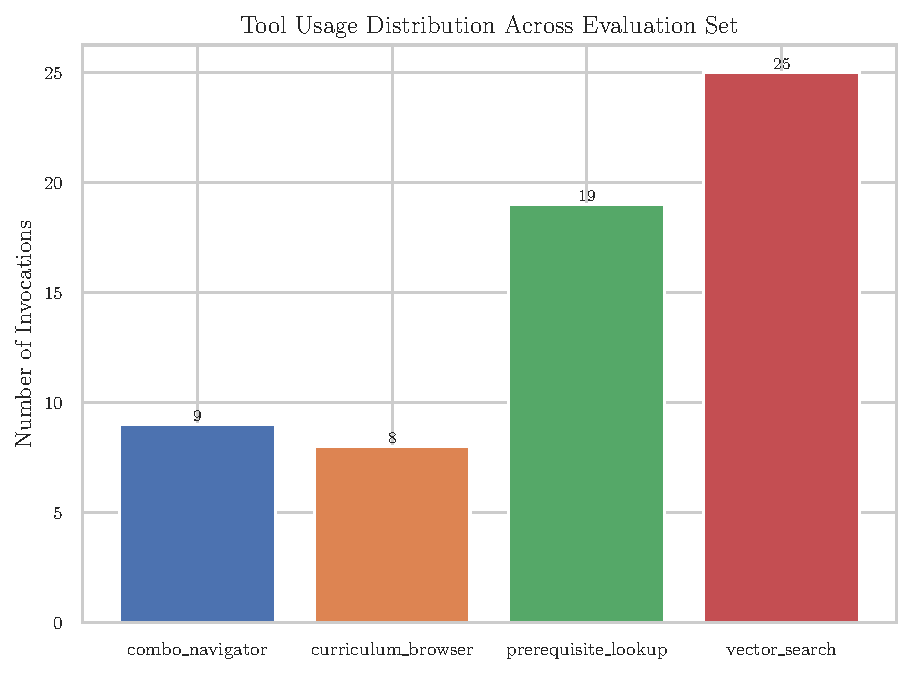
\includegraphics[width=\columnwidth]{tool_usage.pdf}
\caption{Tool usage distribution across the 48 evaluation questions.}
\label{fig:tools}
\end{figure}

\texttt{vector\_search} is the most frequently invoked tool, used for content questions, assessment details, and learning outcomes. \texttt{prerequisite\_lookup} and \texttt{curriculum\_browser} are used for structured queries about dependencies and semester plans. \texttt{combo\_navigator} is invoked less frequently, corresponding to the smaller number of combo/pathway questions in the test set.

\subsection{Per-Question Analysis}

Fig.~\ref{fig:delta} shows the per-question correctness delta (RAG minus baseline) across all 48 questions.

\begin{figure}[!t]
\centering
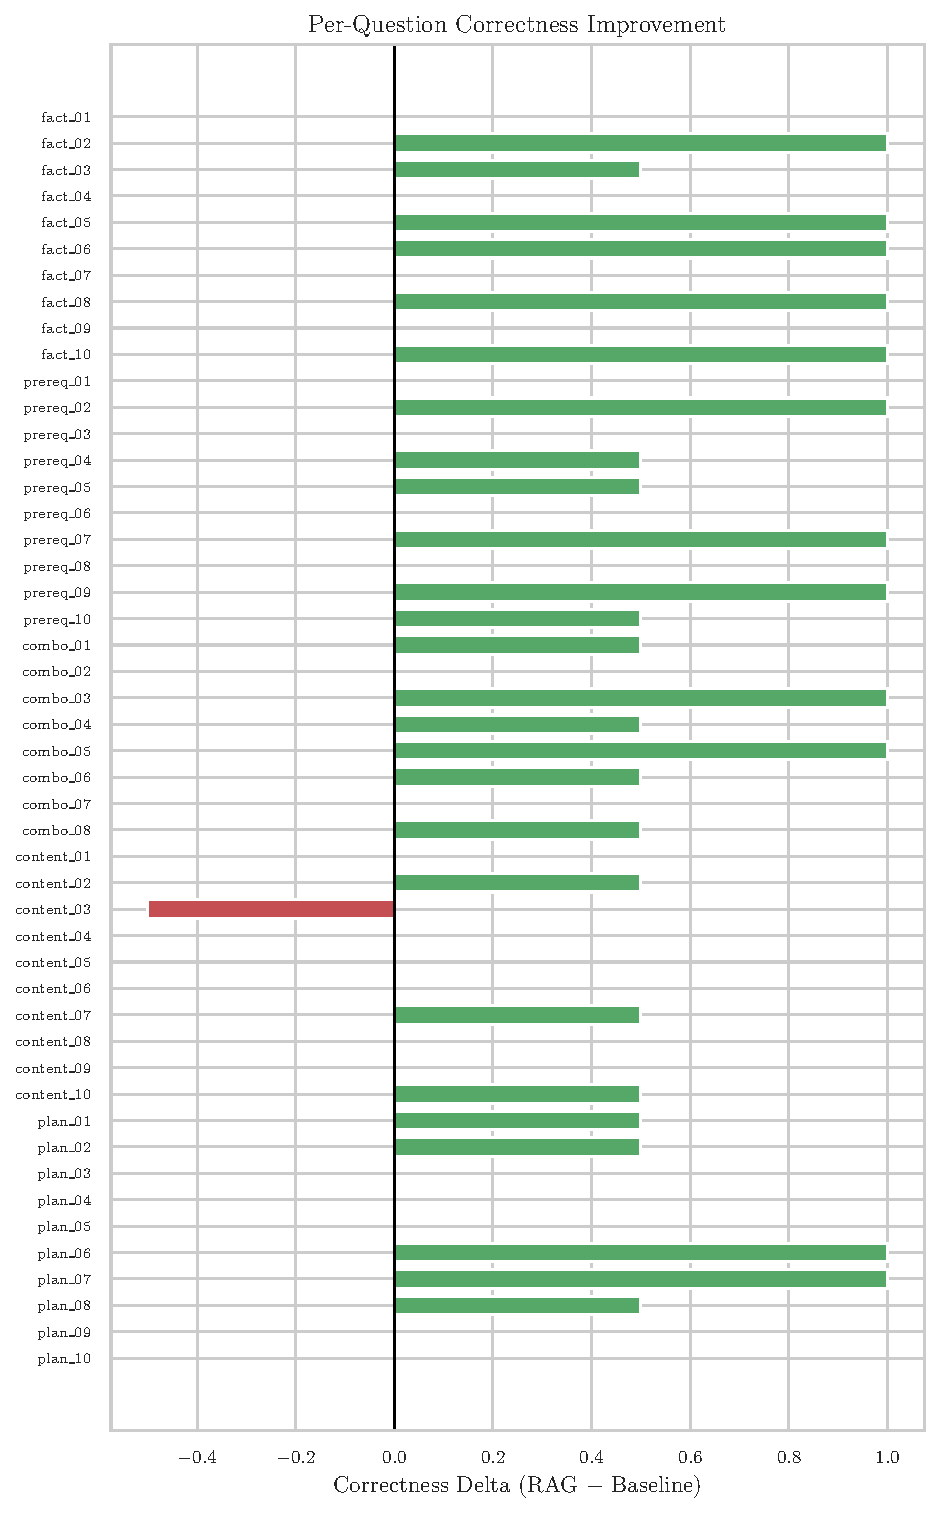
\includegraphics[width=\columnwidth,height=0.85\textheight,keepaspectratio]{per_question_delta.pdf}
\caption{Per-question correctness improvement ($\Delta$ = RAG $-$ Baseline). Positive values (green) indicate RAG outperformance; negative values (red) indicate baseline outperformance.}
\label{fig:delta}
\end{figure}

The majority of questions show zero or positive delta, with 29 questions showing improvement from RAG and only 2 questions where the baseline outperforms. The 17 remaining questions have equal scores for both systems.

\subsection{Failure Analysis}

We identify three failure modes in the RAG system:

\textbf{Credit value confusion} (fact\_01, fact\_04, fact\_09): The system occasionally returns incorrect credit values when the \texttt{vector\_search} tool retrieves chunks that do not contain the credit field, and the \texttt{curriculum\_browser} is not invoked as a fallback.

\textbf{Incomplete prerequisite chains} (prereq\_03, prereq\_06): Deep prerequisite hierarchies spanning 3+ levels are sometimes partially resolved, with intermediate requirements omitted.

\textbf{Cross-document synthesis} (content\_03, content\_09): Questions requiring information from multiple unrelated documents (e.g., comparing assessment methods of two courses) perform worst, as the vector search must be invoked multiple times and the retrieved chunks may not cover all relevant aspects.

The baseline system exhibits systematic failures: inventing nonexistent course codes, assigning incorrect semester numbers (e.g., semester 6 instead of 4), and reporting inaccurate credit totals (40 subjects instead of 47).

% ======================================================================
\section{Discussion}

\subsection{Why Structured Tools Over Graph RAG}

An initial design proposal suggested Graph RAG for this project, given the relational nature of curriculum data (prerequisite dependencies, combo groupings, semester ordering). We chose standard RAG with structured JSON lookup tools for three reasons:

\begin{enumerate}
    \item \textbf{Small corpus}: With only 9 source documents and 47 courses, the overhead of building and maintaining a knowledge graph is not justified.
    \item \textbf{Explicit relationships}: Prerequisites are enumerated in tables, not implied by context. A JSON lookup with recursive chain resolution handles them deterministically, avoiding the probabilistic nature of graph traversal over embeddings.
    \item \textbf{Evaluation clarity}: Deterministic tools produce verifiable outputs, making correctness evaluation straightforward.
\end{enumerate}

The evaluation results support this decision: structured tools (\texttt{prerequisite\_lookup}, \texttt{curriculum\_browser}, \texttt{combo\_navigator}) achieve higher per-question correctness than \texttt{vector\_search} on their respective question categories.

\subsection{Multi-Tool Iteration}

A key architectural contribution is the multi-tool loop. The original single-pass design (agent $\rightarrow$ tool $\rightarrow$ generate) could only invoke one tool per question. Complex queries such as ``Can I accelerate to Deep Learning?'' require both \texttt{prerequisite\_lookup} (to resolve the dependency chain) and \texttt{curriculum\_browser} (to identify semester placements). The looping design allows the agent to gather all necessary data before synthesis.

\subsection{Document Grading and Query Rewriting}

The grading step is applied only to \texttt{vector\_search} results, as structured tools return deterministic data that is always relevant. When vector search results are judged irrelevant, the query is rewritten once. We observed that the rewriter sometimes expands partial course codes incorrectly (e.g., ``MAE'' $\rightarrow$ ``Master of Arts in Education''), which we mitigated by adding explicit instructions to preserve course code prefixes.

\subsection{Limitations}

The system has several limitations:
\begin{itemize}
    \item The evaluation uses LLM-as-judge rather than human evaluation. While prior work shows high correlation between LLM and human judgments~\cite{ref_llm_judge}, bias from the same model family (GPT-4o-mini) evaluating its own outputs cannot be ruled out.
    \item The test set of 48 questions, while covering five categories, is relatively small. A larger evaluation set would provide more statistical confidence.
    \item The system covers only the K20-K21 curriculum version. Extending to multiple curriculum versions would require versioned structured tables.
    \item Cross-document questions remain challenging, suggesting that the single-query vector search approach is insufficient for multi-source synthesis tasks.
\end{itemize}

% ======================================================================
\section{Conclusion}

We presented an agentic RAG system for university curriculum navigation that combines semantic vector search with deterministic structured lookup tools. The LangGraph-based agent can iteratively invoke multiple tools, grade document relevance, and rewrite queries before synthesizing a final answer. Evaluated on a 48-question test set, the system achieves 0.625 correctness compared to 0.240 for an LLM-only baseline (+160.4\% relative), with faithfulness improving from 0.000 to 0.865. The largest gains appear in factual lookup and specialization pathway questions, where deterministic tools provide precise answers that the baseline model would otherwise hallucinate.

Future work includes extending the evaluation with human judges, supporting multiple curriculum versions, improving cross-document retrieval through multi-hop strategies, and deploying the system for real student use with feedback collection.

\section*{Acknowledgments}
This work was conducted as part of the BIT\_AI program at FPT University.

\begin{thebibliography}{10}
\bibliographystyle{IEEEtran}

\bibitem{ref_rag_survey}
Y.~Gao, Y.~Xiong, X.~Xu, et al., ``Retrieval-Augmented Generation for Large Language Models: A Survey,'' \textit{arXiv preprint arXiv:2312.10997}, 2023.

\bibitem{ref_lewis_rag}
P.~Lewis, E.~Perez, A.~Piktus, et al., ``Retrieval-Augmented Generation for Knowledge-Intensive NLP Tasks,'' in \textit{Proc. NeurIPS}, 2020, pp.\ 9459--9474.

\bibitem{ref_langgraph}
LangChain, ``LangGraph: Build stateful, multi-actor applications with LLMs,'' 2024. [Online]. Available: \url{https://github.com/langchain-ai/langgraph}

\bibitem{ref_react}
S.~Yao, J.~Zhao, D.~Yu, et al., ``ReAct: Synergizing Reasoning and Acting in Language Models,'' in \textit{Proc. ICLR}, 2023.

\bibitem{ref_llm_judge}
L.~Zheng, W.-L.~Chiang, Y.~Sheng, et al., ``Judging LLM-as-a-Judge with MT-Bench and Chatbot Arena,'' in \textit{Proc. NeurIPS}, 2023.

\bibitem{ref_reranking}
N.~Nogueira, W.~Jiang, R.~Pradeep, and J.~Lin, ``Document Ranking with a Pretrained Sequence-to-Sequence Model,'' in \textit{Proc. Findings of EMNLP}, 2020, pp.\ 708--718.

\bibitem{ref_edu_ai}
K.~R.~Koedinger and A.~Corbett, ``Cognitive Tutors: Technology Bringing Learning Sciences to the Classroom,'' in \textit{The Cambridge Handbook of the Learning Sciences}, 2nd ed., R.~K.~Sawyer, Ed. Cambridge Univ.\ Press, 2014, pp.\ 61--78.

\end{thebibliography}

\vfill

\end{document}
